\documentclass[preview]{standalone}

\usepackage{amsmath}
\usepackage{amssymb}
\usepackage{stellar}
\usepackage{wrapfig}
\usepackage{bettelini}

\hypersetup{
    colorlinks=true,
    linkcolor=black,
    urlcolor=blue,
    pdftitle={Stellar},
    pdfpagemode=FullScreen,
}

\begin{document}

\id{biologia-evoluzione-uomo}
\genpage

\section{Classificazione di Homo sapiens}

\begin{snippetdefinition}{paleoantropologia-definition}{Paleoantropologia}
    La \textit{paleoantropologia} è una disciplina dell'antropologia che studia la storia evolutiva
    dell'essere umano.
\end{snippetdefinition}

\begin{snippetdefinition}{mammiferi-definition}{Mammiferi}
    I \textit{mammiferi} sono una classe di vertebrati caratterizzata dall'allattamento della prole. 
\end{snippetdefinition}

\begin{snippetdefinition}{primati-definition}{Primati}
    I \textit{primati} sono un ordine di mammiferi placentati i cui rappresentanti
    più diffusi sono i tarsi, i lemuri e le scimmie, tra cui l'essere umano moderno. 
\end{snippetdefinition}

\plain{L'Homo sapiens è caratterizzato dalle seguenti proprietà:}

\begin{snippet}{classificazione-homo-sapiens}
    \vspace{0.25cm}
    \begin{center}
        \begin{tabular}{|l|l|}
            \hline Dominio & Eukarya \\
            \hline Regno & Animalia \\
            \hline Phylum & Chordata \\
            \hline Subphylum & Vertebrata \\
            \hline Classe & Mammalia \\
            \hline Ordine & Primates \\
            \hline Superfamiglia & Hominoidea \\
            \hline Famiglia & Hominidae \\
            \hline Sottofamiglia & Homininae \\
            \hline Genere & Homo \\
            \hline Specie & H. sapiens \\
            \hline
        \end{tabular}
    \end{center}
    \vspace{0.25cm}
\end{snippet}

\begin{snippet}{evoluzione-umana-expl1}
    La storia dell'evoluzione umana è iniziata in Africa tra
    7 e 6 milioni di anni fa, quando la linea evolutiva dell'uomo
    si è separata da quella dello scimpanzé. 
\end{snippet}

\begin{snippetdefinition}{scimmie-antropomorfe-definition}{Scimmie antropomorfe}
    Le \textit{sciemmie antropomorfe} comprendono i gibboni, gli oranghi, i gorilla
    e gli scimpanzé (grandi scimmie).
\end{snippetdefinition}

\begin{snippetdefinition}{ominidi-definition}{Ominidi}
    Gli \textit{ominidi} sono una famiglia di primati
    alla quale appartengono gli esseri umani
    e gran parte delle scimmie antropomorfe. % oranghi, gorilla, scimpanzè
\end{snippetdefinition}

\begin{snippetdefinition}{ominoidei-definition}{Ominoidei}
    La categoria degli \textit{ominoidei} include scimmie antropomorfe ed esseri umani.
    Essa comprende gli ominidi e i gibboni.
\end{snippetdefinition}

\begin{snippetdefinition}{antropoidi-definition}{Scimmie antropoidi}
    Gli \textit{antropoidi} sono un gruppo di primati che comprende le
    scimmie e gli ominoidei. 
\end{snippetdefinition}

\begin{snippetdefinition}{ominini-definition}{Ominini}
    Gli \textit{ominini} sono una tribù all'interno della famiglia degli ominidi
    che comprende la linea evolutiva che ha portato agli esseri umani,
    includendo gli antenati diretti e gli scimpanzé.
\end{snippetdefinition}

\includesnpt[width=70\%|src=/snippet/static/albero-filogenetico-primati.png]{centered-img}

\begin{snippet}{a893df50-d271-49ba-bdfb-b437fe390a6a}
    Gli adattamenti che portarono all'evoluzione dei primati sono legati alla
    vita arboricola, ovvero:
    \begin{itemize}
        \item estremità prensili;
        \item dominanza della vista;
        \item verticalizzazione del corpo;
        \item aumento delle dimensioni cerebrali;
        \item incremento delle cure parentali.
    \end{itemize}
\end{snippet}

\begin{snippetdefinition}{ardipithecus-definition}{Ardipithecus}
    Gli \textit{ardipitechi} sono un genere estinto di primati appartenenti alla famiglia degli ominini,
    vissuti in Africa.
    Essi vissero fra i 5.6 milioni e 4.4 milioni di anni fa.
\end{snippetdefinition}

\plain{L'ardipithecus è il primo genere di ominini che tendenzialmente inizia a verticalizzarsi.}

\begin{snippetdefinition}{australopithecus-definition}{Australopithecus}
    L'\textit{australopitheco} è un genere estinto di primati della famiglia
    degli ominidi, che si ritiene appartenente alla linea
    evolutiva dell'essere umano e apparso successivamente alla separazione della
    linea che ha condotto ai nostri parenti viventi più prossimi, gli scimpanzé.
    Gli australopithechi vissero tra i 4.2 milioni e 2 milioni di anni fa.
\end{snippetdefinition}

\begin{snippetdefinition}{homo-neanderthalensis-definition}{Homo neanderthalensis}
    L'\textit{uomo di Neandertal} è un ominide strettamente affine all'uomo moderno
    che visse tra i 200 mila e 30 mila anni fa.
\end{snippetdefinition}

\includesnpt[width=70\%|src=/snippet/static/linea-temporale-ominini.png]{centered-img}

\section{Il bipedismo precede lo sviluppo del cervello}

\begin{snippet}{bipedismo-precede-cervello}
    Contrariamente ad alcune ipotesi secondo le quali la verticalizzazione degli
    ominini fosse avvenuta come conseguenza dell'aumento dell'intelligenza,
    sono stati ritrovati fossili di ominini con postura eretta ma cervelli molto piccoli.
\end{snippet}

\begin{snippet}{evoluzione-parto-ominini}
    \setlength{\intextsep}{0pt}%
    \begin{wrapfigure}{r}{8cm}
        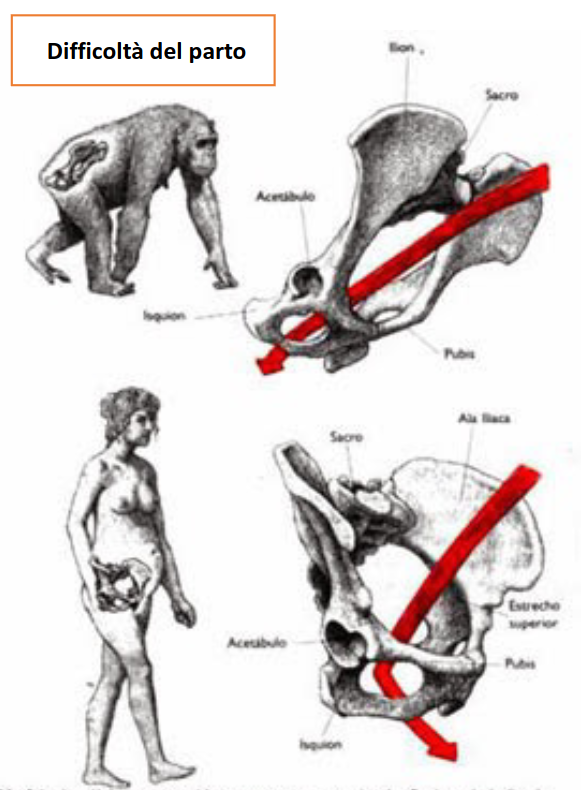
\includegraphics[width=7.5cm]{./resources/difficolta-parto-ominini.png}
        \vspace{-1cm}
    \end{wrapfigure}

    Il parto umano è relativamente difficile rispetto a quello di molti altri mammiferi,
    compresi i nostri parenti più stretti come le scimmie antropomorfe.
    Questo è dovuto in parte all'avvento della postura eretta, che ha portato a notevoli cambiamenti
    anatomici. 

    Con l'evoluzione del genere Homo, il cervello è diventato molto più grande. Un cervello più grande richiede un cranio più grande, il che significa che la testa del bambino è relativamente grande rispetto al canale del parto.
    Da un punto di vista evolutivo questo problema si è risolto favorendo i bambini prematuri, con un cranio più piccolo,
    diminuendo quindi la durata della gestazione.
    \wrapfill
\end{snippet}

\section{Out of Africa}

\begin{snippetdefinition}{out-of-africa-definition}{Out of Africa}
    La teoria \textit{Out of Africa} suggerisce che gli esseri umani moderni abbiano avuto origine in Africa e poi si siano diffusi in tutto il mondo.
\end{snippetdefinition}

\includesnpt[width=70\%|src=/snippet/static/out-of-africa.png]{centered-img}

\begin{snippet}{d4239906-0246-439c-b67f-dbd9625e4f29}
    Gli uomini di Neanderthal erano quindi già in Europa, gli Homo Sapiens
    sono arrivati e a seguito è avvenuta la scomparsa degli uomini di Neandertal.
    Le due specie si sono sicuramente incrociate e vi era anche una convivenza.
\end{snippet}

% TODO: usare ciclo_amminoacidi.png

\end{document}